\documentclass[a4paper,10pt]{article}
\usepackage[utf8]{inputenc}
\usepackage{amsmath}
\usepackage{amssymb}
\usepackage{textcomp}
%\documentclass[a4paper,11pt,notitlepage]{article}
\usepackage[dvips]{graphicx}
%\usepackage{subfigure}
%\usepackage{wrapfig}

\renewcommand\refname{Bibliography}
\usepackage[round]{natbib}
\usepackage{natbibspacing}

\setlength{\parindent}{0pt}
\usepackage{parskip}
% smaller margins:
\usepackage{fullpage}
% smaller font in captions:
%\newcommand{\captionfonts}{\footnotesize}
\usepackage[font=footnotesize,labelfont=bf]{caption}

%\usepackage{german}
\usepackage{eurosym}
\usepackage{wrapfig}


\usepackage[usenames,dvipsnames]{color}
% create color commands
\newcommand{\unsure}[1]{ {\color{Gray} #1} }
\newcommand{\changed}[1]{ {\color{red} #1} }
\newcommand{\mine}[1]{ {\color{blue} #1} }
%\newcommand{\todo}[1]{ {\color{green} #1} }
%\newcommand{\unsure}[1]{ {\gray{ #1} }}

%\usepackage{todonotes}
%\newcommand{\insertref}[1]{\todo[color=green!40]{#1}}
%\newcommand{\explainindetail}[1]{\todo[color=red!40]{#1}}

\usepackage{hyperref}
\definecolor{darkred}{rgb}{0.2,0.0,0.0}
\definecolor{rred}{rgb}{0.7,0.0,0.0}
\hypersetup{colorlinks,breaklinks,
            linkcolor=darkred,urlcolor=darkred,
            anchorcolor=darkred,citecolor=darkred}

\renewcommand{\familydefault}{\sfdefault}

% boxes
\setlength{\fboxsep}{4mm}
%\usepackage{tikz}
%\tikz \node[rectangle, draw=red, thick] {test};






\begin{document}
\title{\textbf{Waveform Comparison - Ring Laser vs. STS-2 Broadband Seismometer}\\
Estimation of Backazimuth and Love Wave Phase Velocity}
\date{}
\maketitle

\section*{Page 1 - Event Information}

\begin{figure}[h!]
\centering
 \fbox{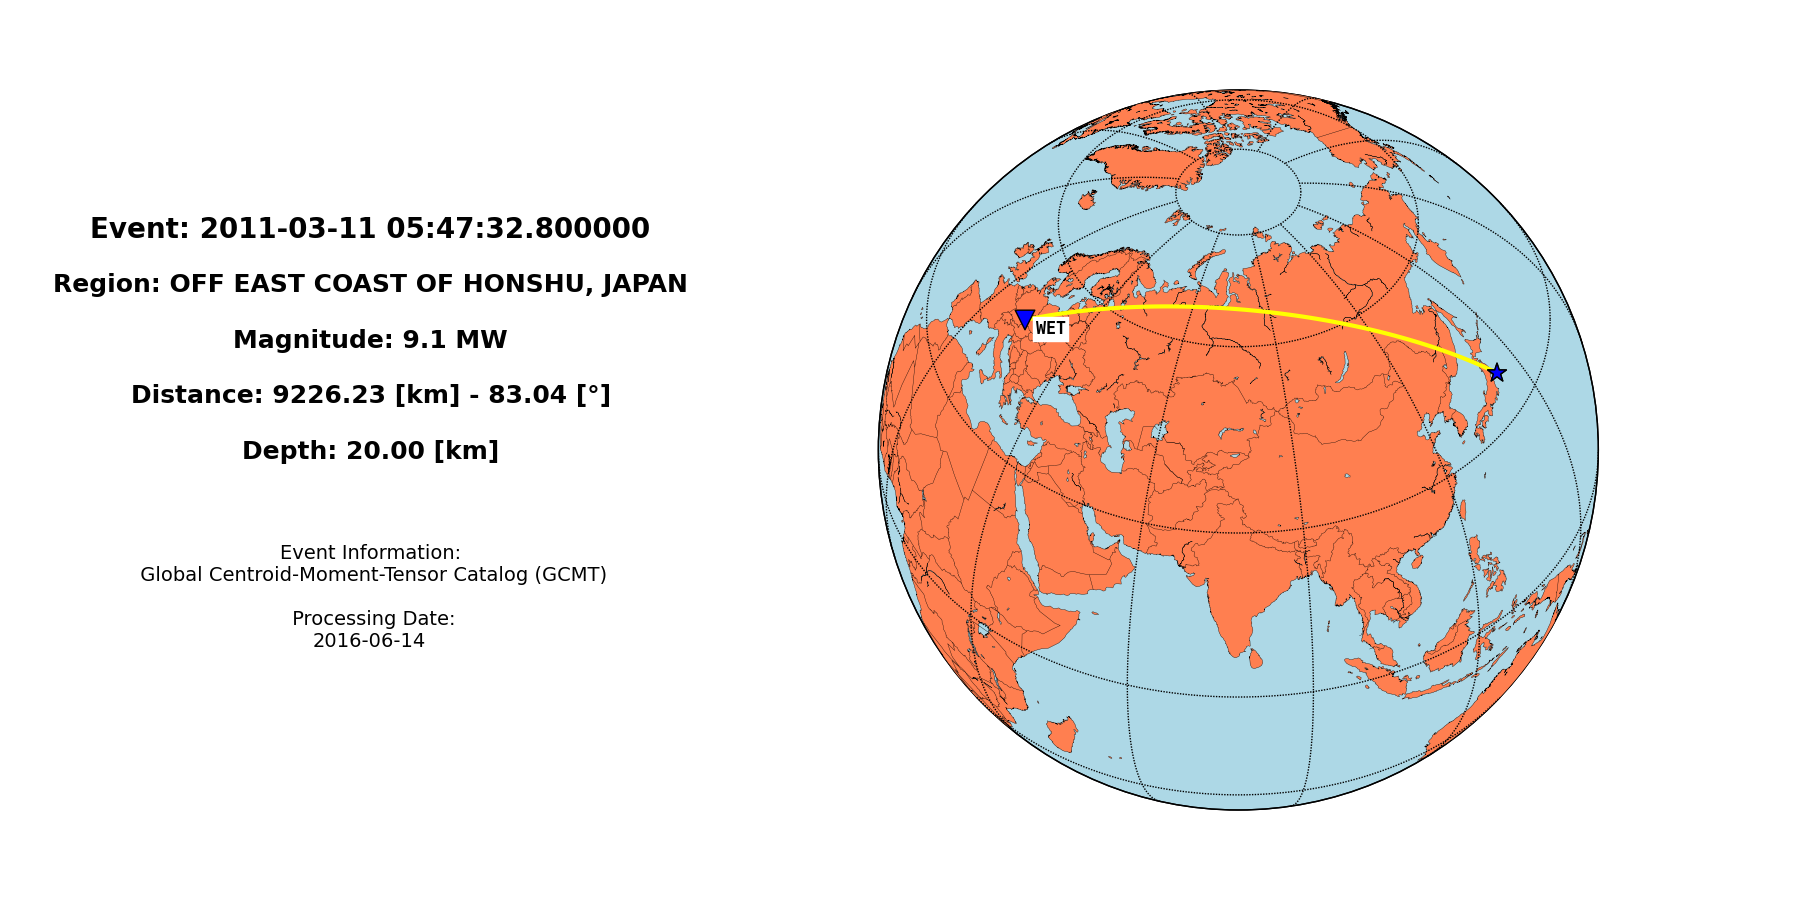
\includegraphics[width=\textwidth]{page_1a.png}}
 \caption{Page 1 - Event Information}
 \label{page1}
\end{figure}

The  first  page  shows  a  map  on  which  the  source  and  receiver  locations  are  indicated.  The  epicenter  of  the source is marked by a blue star, while the marker for the receiver station is a blue triangle with the shortcut of  the  station's  name  next  to  it.  The  scale  of  the  map  depends  on  the  source-receiver  distance  to  allow  for higher resolution for local events.\\
On the left side, registered event information is displayed:

\begin{itemize}
	\item origin time in the format YYYY-mm-dd [T] HH:MM:SS
	\item Flinn-Engdahl region
	\item moment magnitude of the earthquake
	\item epicentral distance (distance between epicenter and receiver station in km and degrees)
	\item depth of the earthquake (distance between epicenter and hypocenter)
\end{itemize}

In the last lines, the source of the event information data is specified.

\newpage

\section*{Page 2 - Waveform Comparison}

\begin{figure}[h!]
\centering
 \fbox{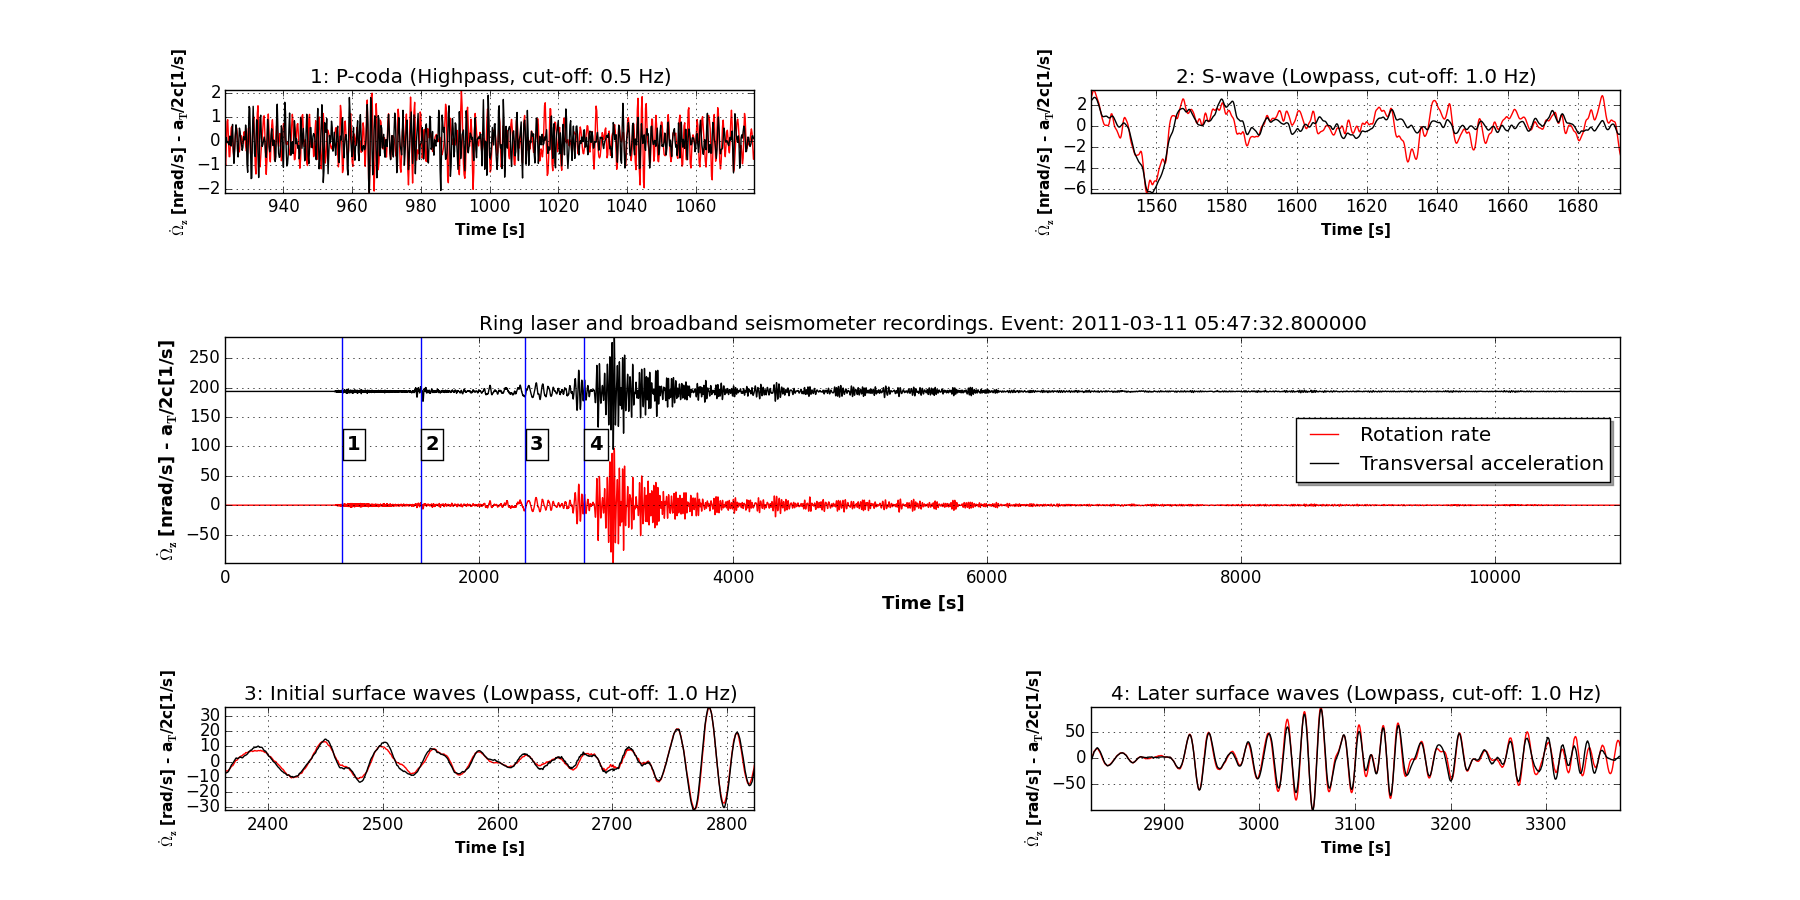
\includegraphics[width=\textwidth]{page_2a.png}}
 \caption{Page 2 - Recordings}
 \label{page2}
\end{figure}

The  recordings  of  the  ring  laser  (red)  and  the  broadband  seismometer  (black)  are  displayed  on  this  page.
The  central  plot  shows  the  complete  traces  that  were  extracted  from  seismometer/ring  laser  recordings  at  the
specified station.  The surrounding four windows represent short time intervals cropped from the trace to distinguish between different parts of the signal.
The start times of these windows are plotted as consecutively numbered vertical lines in the central plot and indicate arrival times of the following wave types (Note: the arrival times were not picked by hand, so they may vary):\\

\begin{tabular}{llll}
	\hspace{2cm} 1. P-wave (P-Coda) & \hspace{4cm} & 2. S-wave & \\
	&&&\\
	\hspace{2cm} 3. Initial surface waves          & \hspace{4cm} & 4. Later surface waves & \\
\end{tabular}

Each signal (rotation rate, acceleration) is detrended linearly, rotation rate units are converted to $\frac{nrad}{s}$. Instrument responses are removed and horizontal acceleration is derived from the particle velocity measurements. Eventually, the signals are low-pass filtered at a certain cutoff-frequency and resampled, depending on the epicentral distance of the event:
\\

\begin{tabular}{l|c|l|l}
	\textbf{Zone} & \textbf{Distance range} &\textbf{ Lowpass cutoff}& \textbf{Resampling (decimation factor)}\\
	\hline
	close events & 0 km $\le$ d $\le$ 333.33 km & 4 Hz & 2 \\
	\hline
	local events & 333.34 km $\le$ d $\le$ 1111.11 km & 2 Hz & 2\\
	\hline
	teleseismic events & d $>$ 1111.11 km & 1 Hz & 4 (P-coda by factor 2)
\end{tabular}
\vspace{.5cm}\\
Also for teleseismic events a bandstop-filter (5s$<$f$<$12s) is applied to wipe out the secondary microseism noise-band. For  displaying  the  transverse  acceleration,  we  need  to  rotate  the  broadband  signal  from  N-/E-components to  radial  and  transverse  components.   In  order  to  achieve  this,  the  N-/E-components  are  rotated  by  the theoretical backazimuth (source direction angle), calculated from the  source-receiver geometry.

Rotation rate (red) and transverse acceleration (black) are shown in the subplots.  The resemblance/coherence of the waveforms depends on the quality of the signals (influenced by magnitude, source-receiver distance, depth) and the accuracy of the theoretical backazimuth.

\newpage
\section*{Page 3 - Velocity and Backazimuth Estimation}

\begin{figure}[h!]
\centering
 \fbox{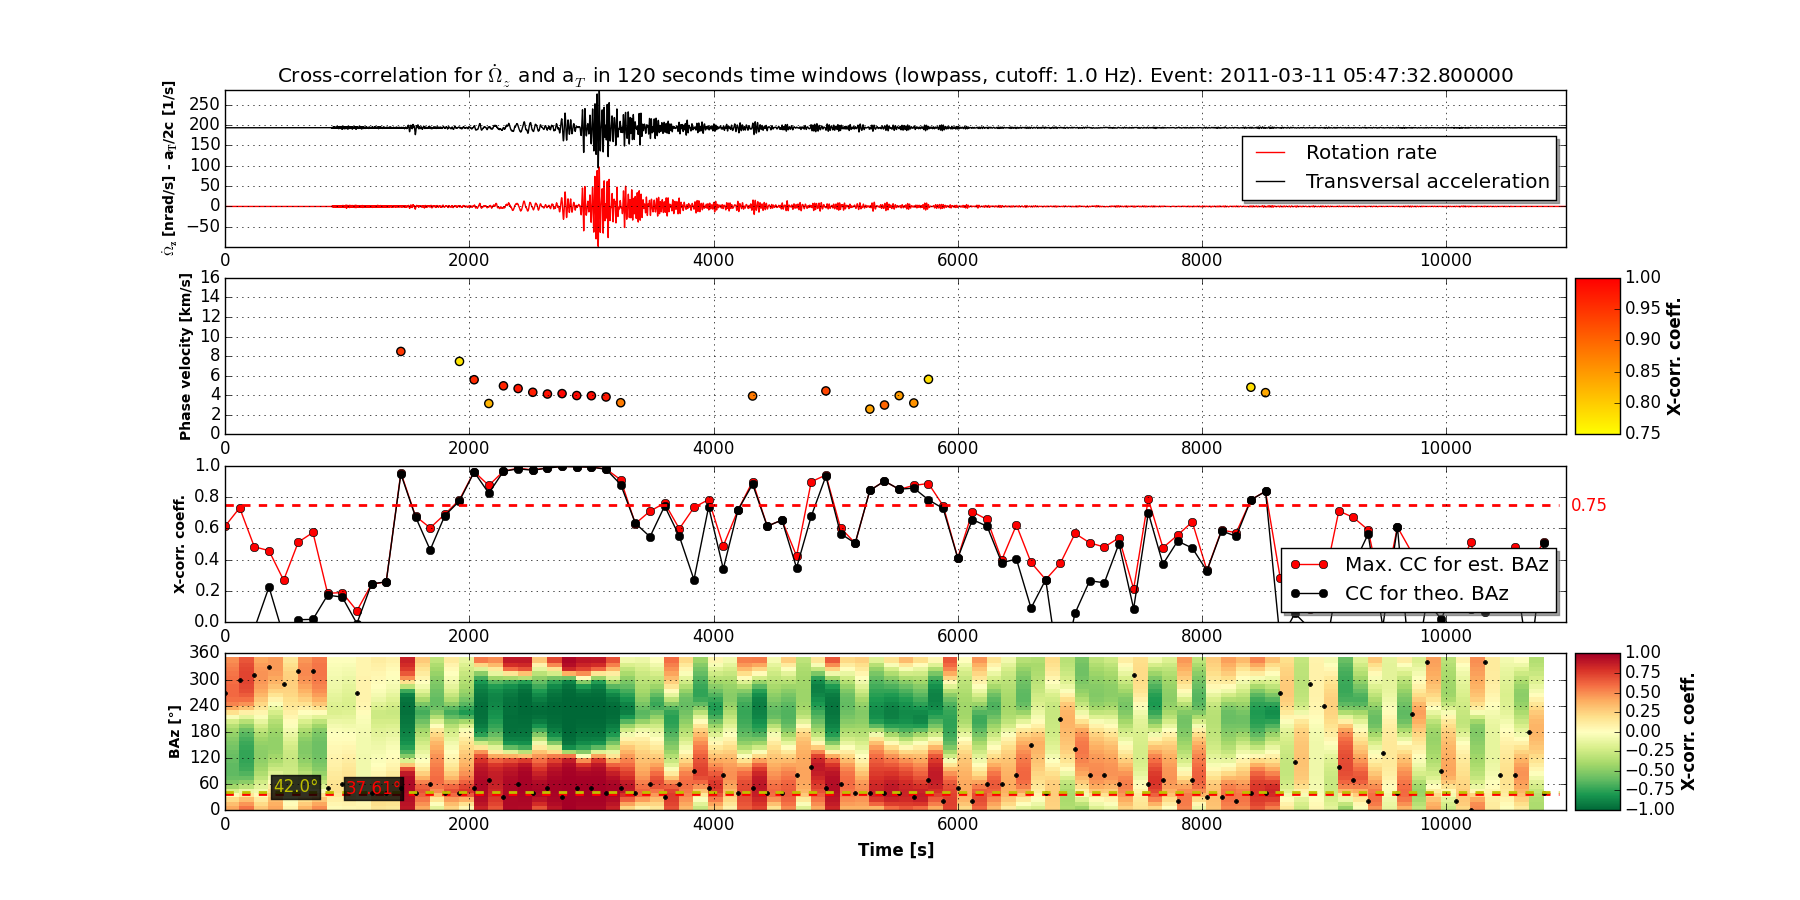
\includegraphics[width=\textwidth]{page_3a.png}}
 \caption{Page 3 - Estimation of Love Wave Phase Velocities and Backazimuth }
 \label{page3}
\end{figure}

Results of the comparison of broadband and rotational signal are shown on this page. The relation between rotation rate and transverse acceleration is used to estimate phase velocities in the signal [cf. \textit{Igel et al.} (2005)]:\\

\begin{equation}
	v_{ph} = \frac{1}{2} \cdot \frac{\alpha_T}{\dot{\Omega_z}}
\end{equation}

In addition, the backazimuth (BAz) is re-evaluated to cross-check the reliability of the theoretical estimation with an estimation from the seismometer/ring laser recordings.\\
The first plot is adopted from the second page and contains the deduced transverse acceleration (black) and
the rotation rate (red) of the station recordings.\\
In order to evaluate the backazimuths and phase velocities, the recordings are divided into sub-intervals whose length depends on the epicentral distance:

\begin{table}[h!]
	\centering
	\begin{tabular}{lc}
		\textbf{Zone} & \textbf{Interval length}\\
		\hline
		close events & 3 s\\
		local events & 5 s\\
		non-local events & 120 s
	\end{tabular}
\end{table}


For each time interval a correlation between transverse acceleration and rotation rate is computed and displayed in the third subplot. Only if this correlation coefficient for a time window exceeds a threshold of 0.75, a \textbf{phase velocity} value is calculated according to equation (1) using the theoretical BAz for rotating the horizontal accelerations (second subplot with a color scale indicating the coefficient value).\\
In order to calculate the best fitting BAz from the observed signals, a grid search optimization algorithm is employed:\\
Essentially, in each interval the program loops through 360\textdegree{} in backazimuth test steps (10\textdegree{} each). In each loop, the algorithm performs a cross-correlation to calculate correlation coefficients (CC) between the rotation rate measurements (ring laser) and the transverse acceleration (broadband seismometer) that is rotated from N-/E-component to radial/transverse by the test step values.\\
The 36 correlation coefficients are plotted column-wise (one column per time interval) in subplot 4, where red fields mark high (positive) correlation, while green ones mark anti-correlation for the associated BAz rotation angle and yellow represents no correlation of the signals. Maximum correlation coefficients of each time interval are displayed as black dots on the respective BAz-field. For comparison, these maximum CCs are also plotted in subplot 3 (red dotted line).\\
In a last step, the routine is re-run for a smaller BAz step-size of 1\textdegree{} and shorter time-windows (30~s) to calculate a more precise estimate of the backazimuth (plotted as yellow dashed line). The estimated BAz value is averaged not over the BAz of all time windows, but only over those for which a CC$>$ 0.9 could be gained.
For comparison, the theoretical BAz is denoted by a red dashed line. 

\section*{Page 4 - P-Coda Evaluation}

\begin{figure}[h!]
\centering
 \fbox{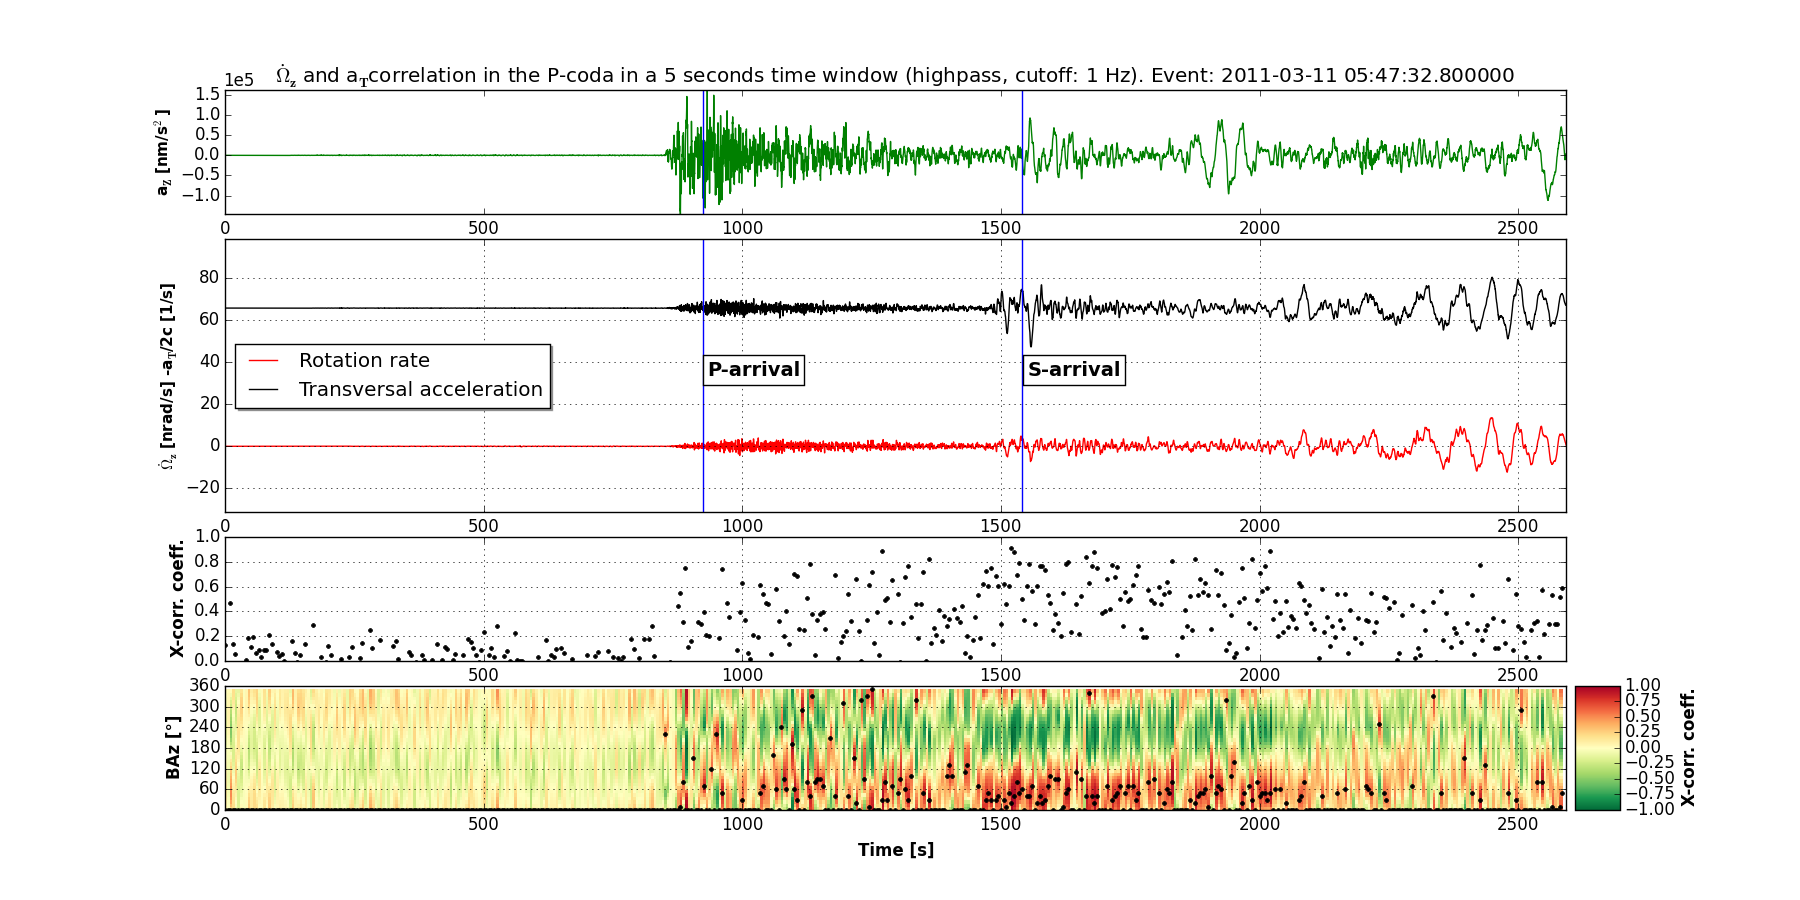
\includegraphics[width=\textwidth]{page_4a.png}}
 \caption{Page 4 - Backazimuth Estimation of the P-coda}
 \label{page4}
\end{figure}

The last page deals particularly with the backazimuth analysis of the P-coda [cf. \textit{Pham et al.}(2009)]. In that context, an interval length of 2 s is used for the cross-correlation windows in the BAz determination algorithm.\\

The uppermost plot shows a time series with the Z-component recordings of the broadband seismometer for the first part of the event.  For the same interval, the rotation rate (red) and transverse acceleration (black) are displayed in the second subplot.  P- and S-wave arrivals are indicated by vertical lines (not picked by hand).\\
For this period, the backazimuth values are estimated via grid search optimization analogous to the processing
before, but at a higher resolution (2~s-windows).\\
The correlation coefficients associated with rotation around the theoretical BAz for each 2~s-interval are plotted
in the third plot (black dots), while the estimated backazimuths (with correlation-coefficients) can be found in
the lowermost figure.  In this plot, black dots mark all the BAz values associated with correlation coefficients
larger than 50\%.
\newpage

\section*{JSON-file}
In the .json-file, processed data is stored for post-processing. The file contains the following information:

\begin{itemize}
	\item data source information (client, network, station, ...)
	\item event identification
	\item start- and endtime
	\item station location (latitude, longitude)
	\item epicentral distance)
	\item moment magnitude
	\item source depth
	\item peak transverse acceleration
	\item peak transverse displacement
	\item peak vertical acceleration
	\item peak rotation rate
	\item peak correlation coefficient
	\item frequency at peak vertical rotation rate
	\item theoretical backazimuth
	\item estimated backazimuth
	\item maximum correlation coefficient for estimated BAz
	\item SNR of transverse acceleration
	\item SNR of vertical acceleration
	\item SNR of vertical rotation rate
	\item mean phase velocities for 8 frequency bands  (0.01-0.02  Hz,  0.02-0.04  Hz,  0.04-0.1  Hz,  0.1-0.2  Hz, 0.2-0.3 Hz, 0.3-0.4 Hz, 0.4-0.6 Hz, 0.6-1 Hz)
	\item standard deviations for these phase velocities
\end{itemize}

\vspace{5cm}
\hrule
\textbf{References:}

\textsc{Igel}, H., U. Schreiber, A. Flaws, B. Schubert, A. Velikoseltsev, and A. Cochard (2005), 
\textit{Rotational Motions induced by the M8.1 Tokashi-oki Earthquake, September 25, 2003}, Geophys.  Res.  Lett. \textbf{32}, L08309.


\textsc{Pham}, N. D., H. Igel, J. Wassermann, M. K{\"a}ser, J. de la Puente, and U. Schreiber (2009), \textit{Observations and Modeling of Rotational Signals in the P-Coda: Constraints on Crustal Scattering}, Bull.  Seismol.  Soc.  Am., \textbf{99}, 1315-1332.



\end{document}
